% Copyright 2004 by Till Tantau <tantau@users.sourceforge.net>.
%
% In principle, this file can be redistributed and/or modified under
% the terms of the GNU Public License, version 2.
%
% However, this file is supposed to be a template to be modified
% for your own needs. For this reason, if you use this file as a
% template and not specifically distribute it as part of a another
% package/program, I grant the extra permission to freely copy and
% modify this file as you see fit and even to delete this copyright
% notice. 

\documentclass{beamer}
\usepackage{graphicx}
\usepackage{amssymb}
\usepackage[encapsulated]{CJK}
% There are many different themes available for Beamer. A comprehensive
% list with examples is given here:
% http://deic.uab.es/~iblanes/beamer_gallery/index_by_theme.html
% You can uncomment the themes below if you would like to use a different
% one:
%\usetheme{AnnArbor}
%\usetheme{Antibes}
%\usetheme{Bergen}
%\usetheme{Berkeley}
%\usetheme{Berlin}
%\usetheme{Boadilla}
%\usetheme{boxes}
%\usetheme{CambridgeUS}
%\usetheme{Copenhagen}
%\usetheme{Darmstadt}
%\usetheme{default}
%\usetheme{Frankfurt}
%\usetheme{Goettingen}
%\usetheme{Hannover}
%\usetheme{Ilmenau}
%\usetheme{JuanLesPins}
%\usetheme{Luebeck}
\usetheme{Madrid}
%\usetheme{Malmoe}
%\usetheme{Marburg}
%\usetheme{Montpellier}
%\usetheme{PaloAlto}
%\usetheme{Pittsburgh}
%\usetheme{Rochester}
%\usetheme{Singapore}
%\usetheme{Szeged}
%\usetheme{Warsaw}

\title{Classification}

% A subtitle is optional and this may be deleted
\subtitle{Cats And Dogs}

\author{Team9}

\date{Presentation , 2019}
% - Either use conference name or its abbreviation.
% - Not really informative to the audience, more for people (including
%   yourself) who are reading the slides online

\subject{Theoretical Computer Science}
% This is only inserted into the PDF information catalog. Can be left
% out. 

% If you have a file called "university-logo-filename.xxx", where xxx
% is a graphic format that can be processed by latex or pdflatex,
% resp., then you can add a logo as follows:

% \pgfdeclareimage[height=0.5cm]{university-logo}{university-logo-filename}
% \logo{\pgfuseimage{university-logo}}

% Delete this, if you do not want the table of contents to pop up at
% the beginning of each subsection:
\AtBeginSubsection[]
{
  \begin{frame}<beamer>{Outline}
    \tableofcontents[currentsection,currentsubsection]
  \end{frame}
}

% Let's get started
\begin{document}

\begin{frame}
  \titlepage
\end{frame}

\begin{frame}{Outline}
  \tableofcontents
  % You might wish to add the option [pausesections]
\end{frame}



% Section and subsections will appear in the presentation overview
% and table of contents.
\section{Introduction}


\begin{frame}{Introduction to your team}
\begin{CJK*}{UTF8}{bsmi}
  \begin{itemize}
  \item {
    1051433 葛東昇  
  }
  \item {
    1051514 沈家葳
  }
  \item {
    1053344 高浩然
  }
  \item {
    1053348 黃世旻
  }
  \end{itemize}
\end{CJK*}
\end{frame}

\begin{frame}{Introduction to the problem you're trying to solve  }
\begin{CJK*}{UTF8}{bsmi}
  \begin{itemize}
  \item {
    我們的這個專題主要要解決的問題是把一張照片讀進來,並且判斷這一張照片是貓還是狗。
  }
  \end{itemize}
\end{CJK*}
\end{frame}



\section{Methodology}

\begin{frame}{Input of your model }
  \begin{itemize}
  \item {
    My first point.
  }
  \item {
    My second point.
  }
  \end{itemize}
\end{frame}

\begin{frame}{Output of your model }
  \begin{itemize}
  \item {
    My first point.
  }
  \item {
    My second point.
  }
  \end{itemize}
\end{frame}

\begin{frame}{Each layer of your model}
  \begin{itemize}
  \item {
    My first point.
  }
  \item {
    My second point.
  }
  \end{itemize}
\end{frame}

\begin{frame}{How you save your model?}
  \begin{itemize}
  \item {
    My first point.
  }
  \item {
    My second point.
  }
  \end{itemize}
\end{frame}

\begin{frame}{File size of your model }
  \begin{itemize}
  \item {
    My first point.
  }
  \item {
    My second point.
  }
  \end{itemize}
\end{frame}

\begin{frame}{What's your loss functions, and why? }
  \begin{itemize}
  \item {
    My first point.
  }
  \item {
    My second point.
  }
  \end{itemize}
\end{frame}

\begin{frame}{What's your optimizer and the setting of hyperparameter?}
  \begin{itemize}
  \item {
    My first point.
  }
  \item {
    My second point.
  }
  \end{itemize}
\end{frame}




\section{Dataset}


\begin{frame}{The size of your dataset should be larger than 1K }
\begin{CJK*}{UTF8}{bsmi}
  \begin{itemize}
  \item {
The size of our dataset 大小為26.0MB 共有1200個檔案如Fig.\,\ref{fig:1} \\
\begin{figure}[h]
\begin{center}
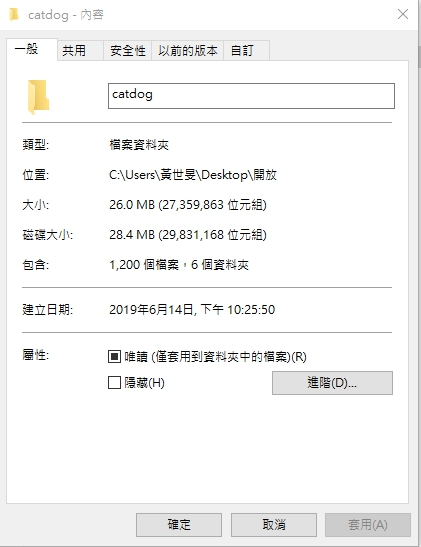
\includegraphics[width=5cm]{dataset.jpg} 
\end{center} 
\label{fig:1} 
\caption{簡易流程圖} 
\end{figure}
  }
  \end{itemize}
\end{CJK*}
\end{frame}

\begin{frame}{How you collect/build your dataset?}
\begin{CJK*}{UTF8}{bsmi}
  \begin{itemize}
  \item {
    Collect:train跟validation的部份我們上kaggle抓裡面的圖片下來用,另外test的部分則是我們自己去拍攝。
  }
  \item {
    Build:將照片中間往外開始剪裁224*224,利用torch內建的tensorflow,將圖片處理成tensor數據。
  }
  \end{itemize}
\end{CJK*}
\end{frame}

\begin{frame}{How many paired training samples in your dataset?}
\begin{CJK*}{UTF8}{bsmi}
  \begin{itemize}
  \item {
    一共是1000張,貓狗各500張。
  }
  \end{itemize}
\end{CJK*}
\end{frame}

\begin{frame}{How many paired validating samples in your dataset?}
\begin{CJK*}{UTF8}{bsmi}
  \begin{itemize}
  \item {
     一共是200張,貓狗各100張。
  }
  \end{itemize}
\end{CJK*}
\end{frame}

\begin{frame}{How many paired testing samples in your dataset?}
\begin{CJK*}{UTF8}{bsmi}
  \begin{itemize}
  \item {
    一共是20張,貓狗各10張。
  }
  \end{itemize}
\end{CJK*}
\end{frame}




\section{ Experimental Evaluation }

\begin{frame}{Experimental environment}
\begin{CJK*}{UTF8}{bsmi}
  \begin{itemize}
  \item {
    我們所測試的環境是在GPU下進行測試。
  }
  \end{itemize}
\end{CJK*}
\end{frame}

\begin{frame}{How many epochs you set for training?}
\begin{CJK*}{UTF8}{bsmi}
  \begin{itemize}
  \item {
   我們總共設了10個epochs來做training的部分。
  }
  \end{itemize}
\end{CJK*}
\end{frame}

\begin{frame}{Qualitative evaluation }
  \begin{itemize}
  \item {
    My first point.
  }
  \item {
    My second point.
  }
  \end{itemize}
\end{frame}

\begin{frame}{Quantitative evaluation }
  \begin{itemize}
  \item {
    My first point.
  }
  \item {
    My second point.
  }
  \end{itemize}
\end{frame}


% Placing a * after \section means it will not show in the
% outline or table of contents.
\section*{Summary}

\begin{frame}{Summary}
  \begin{itemize}
  \item
    The \alert{first main message} of your talk in one or two lines.
  \item
    The \alert{second main message} of your talk in one or two lines.
  \item
    Perhaps a \alert{third message}, but not more than that.
  \end{itemize}
  
  \begin{itemize}
  \item
    Outlook
    \begin{itemize}
    \item
      Something you haven't solved.
    \item
      Something else you haven't solved.
    \end{itemize}
  \end{itemize}
\end{frame}



\end{document}


